\XtoCBlock{TDSystemO1}
\label{block:TDSystemO1}
\begin{figure}[H]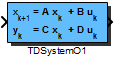
\includegraphics{TDSystemO1}\end{figure} 

\begin{XtoCtabular}{Inports}
In & Input \#1\tabularnewline
\hline
\end{XtoCtabular}


\begin{XtoCtabular}{Outports}
Out & Output \#1\tabularnewline
\hline
\end{XtoCtabular}

\begin{XtoCMaskParamTabular}{Mask Parameters}
\rowcolor[gray]{0.8}\textbf{Name} & \textbf{ID} & \textbf{Description}\tabularnewline\hline
A & 1 & State matrix A\tabularnewline
\hline
B & 2 & Input matrix B\tabularnewline
\hline
C & 3 & Output matrix C\tabularnewline
\hline
D & 4 & Feedthrough matrix D\tabularnewline
\hline
\end{XtoCMaskParamTabular}

\subsubsection*{Description:}
1st order time discrete system with one input and one output.

% include optional documentation file
\InputIfFileExists{\XcHomePath/Library/Control/Doc/TDSystemO1_Info.tex}{\vspace{1ex}}{}

\subsubsection*{Implementations:}
\begin{tabular}{l l}
\textbf{FiP8} & 8 Bit Fixed Point Implementation\tabularnewline
\textbf{FiP16} & 16 Bit Fixed Point Implementation\tabularnewline
\textbf{FiP32} & 32 Bit Fixed Point Implementation\tabularnewline
\textbf{Float32} & 32 Bit Floating Point Implementation\tabularnewline
\textbf{Float64} & 64 Bit Floating Point Implementation\tabularnewline
\end{tabular}

\XtoCImplementation{FiP8}
\nopagebreak[0]

8 Bit Fixed Point Implementation

\begin{XtoCtabular}{Inports Data Type}
In & int8\tabularnewline
\hline
\end{XtoCtabular}

\begin{XtoCtabular}{Outports Data Type}
Out & int8\tabularnewline
\hline
\end{XtoCtabular}

\ifdefined \AddTestReports
\InputIfFileExists{\XcHomePath/Library/Control/Doc/Test-Results/Test_TDSystemO1_FiP8.tex}{}{}
\fi
\XtoCImplementation{FiP16}
\nopagebreak[0]

16 Bit Fixed Point Implementation

\begin{XtoCtabular}{Inports Data Type}
In & int16\tabularnewline
\hline
\end{XtoCtabular}

\begin{XtoCtabular}{Outports Data Type}
Out & int16\tabularnewline
\hline
\end{XtoCtabular}

\ifdefined \AddTestReports
\InputIfFileExists{\XcHomePath/Library/Control/Doc/Test-Results/Test_TDSystemO1_FiP16.tex}{}{}
\fi
\XtoCImplementation{FiP32}
\nopagebreak[0]

32 Bit Fixed Point Implementation

\begin{XtoCtabular}{Inports Data Type}
In & int32\tabularnewline
\hline
\end{XtoCtabular}

\begin{XtoCtabular}{Outports Data Type}
Out & int32\tabularnewline
\hline
\end{XtoCtabular}

\ifdefined \AddTestReports
\InputIfFileExists{\XcHomePath/Library/Control/Doc/Test-Results/Test_TDSystemO1_FiP32.tex}{}{}
\fi
\XtoCImplementation{Float32}
\nopagebreak[0]

32 Bit Floating Point Implementation

\begin{XtoCtabular}{Inports Data Type}
In & float32\tabularnewline
\hline
\end{XtoCtabular}

\begin{XtoCtabular}{Outports Data Type}
Out & float32\tabularnewline
\hline
\end{XtoCtabular}

\ifdefined \AddTestReports
\InputIfFileExists{\XcHomePath/Library/Control/Doc/Test-Results/Test_TDSystemO1_Float32.tex}{}{}
\fi
\XtoCImplementation{Float64}
\nopagebreak[0]

64 Bit Floating Point Implementation

\begin{XtoCtabular}{Inports Data Type}
In & float64\tabularnewline
\hline
\end{XtoCtabular}

\begin{XtoCtabular}{Outports Data Type}
Out & float64\tabularnewline
\hline
\end{XtoCtabular}

\ifdefined \AddTestReports
\InputIfFileExists{\XcHomePath/Library/Control/Doc/Test-Results/Test_TDSystemO1_Float64.tex}{}{}
\fi
